\documentclass[conf]{new-aiaa}
%\documentclass[journal]{new-aiaa} for journal papers
\usepackage[utf8]{inputenc}

\usepackage{graphicx}
\usepackage{amsmath}
\usepackage[version=4]{mhchem}
\usepackage{siunitx}
\usepackage{longtable,tabularx}

\usepackage{acro}
\usepackage{algorithm}
\usepackage{algpseudocode}
\usepackage{caption}
\usepackage{subcaption}


\usepackage{hyperref}
\usepackage{pgfplots}
\usepackage{tikz}
\usepackage{ifthen}
\usepackage{multirow}

\usetikzlibrary{matrix,calc}
% \addbibresource{bibs/ieee.bib}

\setlength\LTleft{0pt} 

\title{SeeNN: Leveraging Multimodal Deep Learning for In-Flight Long-Range Atmospheric Visibility Estimation in Aviation Safety}


% Taha Bouhsine {\textsuperscript{*}}, Giuseppina Carannante{\textsuperscript{*}}, Nidhal C. Bouaynaya{\textsuperscript{*}}, Soufiane Idbraim {\textsuperscript{$\dagger$}}, Phuong Tran\IEEEauthorrefmark{4},  Grant Morfit\IEEEauthorrefmark{4}, \\ Maggie Mayfield\IEEEauthorrefmark{4}, and Charles Cliff Johnson \IEEEauthorrefmark{4}
\author{Taha Bouhsine \footnote{Graduate Research Fellow}, Giuseppina Carannante.\footnote{Postdoctoral Fellow}, Nidhal C. Bouaynaya.\footnote{Associate Dean for Research \& Graduate Studies and Professor of Electrical \& Computer Engineering}}
\affil{Electrical and Computer Engineering Department, Henery M.Rowan College of Engineering, Rowan University, Glassboro, New Jersey, 08028}
\author{Soufiane Idbraim \footnote{Computer Science Professor and Head of IRF-SIC Laboratory}}
\affil{IRF-SIC Laboratory, Computer Science Department, Faculty of Sciences Agadir, Ibn Zohr University, Agadir, Morocco}
\author{Phuong Tran, Grant Morfit, Maggie Mayfield, Charles Cliff Johnson}
\affil{William J. Hughes Technical Center, Federal Aviation Administration, Atlantic City, NJ, USA}

\begin{document}

\maketitle

\begin{abstract}
Deep learning (DL) models have attained state-of-the-art performance in numerous fields. Nevertheless, for certain real-world applications, existing models encounter diverse challenges, ranging from a lack of generability to new data to issues of scalability and overfitting. In this context, integrating information extracted from different modalities holds promise as a potential solution to alleviate these challenges.
This paper introduces SeeNN (\url{https://github.com/skywolfmo/seeNN-paper}), a multimodal deep-learning framework for long-range atmospheric visibility estimation. Using multimodal deep learning, SeeNN fuses various modalities to estimate long-range atmospheric visibility. These modalities include RGB imagery, Edge Map, Entropy Map, Depth Map, and Normal Surface Map. Results show that in contrast to single-modality RGB, which achieves only 87.92\% accuracy, multimodal deep learning models achieve an accuracy of over 96\%.
This significant improvement highlights the potential of multimodal approaches to enhance the accuracy and reliability of atmospheric visibility estimation, which is crucial for improving safety in applications such as aviation, maritime navigation, and autonomous vehicles. By addressing challenges such as data variability, environmental factors, and the inherent complexity of atmospheric conditions, SeeNN contributes to more reliable and robust visibility estimation systems, thereby enhancing safety and operational efficiency in critical environments.






\end{abstract}

% \section{Nomenclature}

% {\renewcommand\arraystretch{1.0}
% \noindent\begin{longtable*}{@{}l @{\quad=\quad} l@{}}
% $A$  & amplitude of oscillation \\
% $a$ &    cylinder diameter \\
% $C_p$& pressure coefficient \\
% $Cx$ & force coefficient in the \textit{x} direction \\
% $Cy$ & force coefficient in the \textit{y} direction \\
% c   & chord \\
% d$t$ & time step \\
% $Fx$ & $X$ component of the resultant pressure force acting on the vehicle \\
% $Fy$ & $Y$ component of the resultant pressure force acting on the vehicle \\
% $f, g$   & generic functions \\
% $h$  & height \\
% $i$  & time index during navigation \\
% $j$  & waypoint index \\
% $K$  & trailing-edge (TE) nondimensional angular deflection rate
% \end{longtable*}}


\section{Introduction}

Atmospheric visibility \cite{visibilitybook} is a critical factor in aviation safety \cite{Kulesa2003WEATHERAA, fultz2016fatal, long2022analysis, fujita1977analysis, ramee2021analysis}, directly impacting a pilot's ability to navigate and make critical decisions. The tragic accident involving professional basketball player Kobe Bryant in January 2020 highlights the severe consequences of visibility-related issues. The National Transportation Safety Board (NTSB) report concluded that the pilot's decision to continue visual flight rules (VFR) into instrument meteorological conditions (IMC) led to spatial disorientation and the subsequent crash. This incident underscores the critical need for accurate, real-time visibility estimation in flight.

Visibility estimation in aviation is particularly challenging due to several factors. Currently, pilots rely heavily on their prior knowledge of landmarks and terrain features to gauge visibility \cite{ahlstrom2019assessments}. This dependence on pre-existing knowledge makes automatic estimation complex, as systems must account for varying geographical contexts. Additionally, conditions such as flying inside clouds or encountering rapidly changing weather patterns further complicate the problem, requiring robust and adaptable solutions.

% In an era of rapidly advancing aviation technology and increasing air traffic, ensuring flight safety remains paramount. This paper introduces a groundbreaking multimodal approach to in-flight visibility estimation, leveraging both monocular RGB cameras and additional multimodal data to significantly enhance aviation safety across diverse weather conditions and flight scenarios.

While deep learning methods have shown great promise in solving complex problems, they face challenges such as overfitting, generalization issues, and potential biases. These limitations are particularly evident in single-modality approaches, especially those relying solely on RGB images for visibility estimation across diverse flight conditions. RGB data alone often fails to capture crucial atmospheric properties or account for factors like glare, low-light conditions, or rapid weather changes \cite{Bouhsine2022, AitOuadil2023, li_meteorological_2017, chaabani_estimating_2018, palvanov_dhcnn_2018, choi_automatic_2018, you_relative_2019, li_method_2019, outay_estimating_2021}.

% start your phrase with a what everytime

To address these challenges, multimodal deep learning techniques have emerged as a promising solution. By integrating information from diverse modalities, these approaches enhance model capabilities and overcome the limitations of single-modality systems \cite{liu2018learn, castanedo2013review, molino2021improved, blasch2021machine}. Each modality captures a distinct type of information, often inaccessible through a single modality approach, resulting in a more comprehensive understanding of the environment and more accurate predictions.

The significance of multimodal deep learning solutions in visibility estimation is increasingly recognized \cite{palvanov_visnet_2019, department_of_computer_science_chu_hai_college_of_higher_education_80_castle_peak_road_castle_peak_bay_tuen_mun_nt_hong_kong_meteorology_2020, AitOuadil2023, app11030997, Zhang2023, You2022, Chen2022, Wauben2016, Cheng2018, Zhou2021}. These models can overcome limitations that plague single-modality systems \cite{huang2021makesmultimodallearningbetter}. The integration of multimodal deep learning (Table~\ref{tab:literature_review}) significantly enhances the robustness, safety, and reliability of deep learning solutions, making them particularly well-suited for critical real-world applications where reliability is crucial \cite{6817512, liang2024foundationsmultisensoryartificialintelligence}.



\begin{table}[htbp]
\centering
\caption{Literature Review of Modalities Used in the Literature for On-Ground Atmospheric Visibility Estimation }
\footnotesize
\begin{center}
\begin{tabular}{|p{3cm}|c|c|c|c|c|c|c|}
\hline
\textbf{Modality} & \textbf{\cite{You2022}} & \textbf{\cite{Palvanov2019}} & \textbf{\cite{Zhang2023}} & \textbf{\cite{Chen2022}} & \textbf{\cite{Wauben2016}} & \textbf{\cite{Cheng2018}} & \textbf{\cite{Zhou2021}} \\
\hline
Depth Map &  & & X & & & & \\
\hline
\begin{tabular}[l]{@{}l@{}}Transmission Map\end{tabular}  & X & & X & & X & & \\
\hline
Disparity Map & X & & & & & &  \\
\hline
Entropy & & & & &  & X & X \\
\hline
Edge Detection & & & & & X & &  \\
\hline
\begin{tabular}[l]{@{}l@{}}Contrast Computation\end{tabular}   & & & & & X & & \\
\hline
\begin{tabular}[l]{@{}l@{}}Koschmieder Law\end{tabular} & &  & & & X & & X \\
\hline
FFT & & X & & & & & \\
\hline
Spectral Filter & & X & & & & & \\
\hline
\begin{tabular}[l]{@{}l@{}}Dark Channel\\ Prior\end{tabular} & & & & X & X & & X\\
\hline
\end{tabular}
\label{tab:literature_review}
\end{center}
\end{table}

Despite advances in deep learning for visibility estimation, there remains a significant gap in addressing in-flight visibility. This gap is largely attributable to the scarcity of comprehensive in-flight visibility datasets, which are crucial for training and validating deep learning models in aviation contexts \cite{AitOuadil2023}. Existing datasets concentrate on short-range visibility, offering a limited spectrum of sceneries, and land covers, and are mainly focused on ground-level atmospheric visibility. Moreover, they are predominantly confined to ground-level altitudes, neglecting the variability and complexity introduced by different elevation viewpoints \cite{AitOuadil2023}. This restriction in dataset diversity hampers the development of more universally applicable and robust in-flight visibility estimation models.

In this work, we propose a multimodal framework for training visibility estimation systems to enhance the accuracy, trustworthiness, and robustness of DL models for atmospheric visibility estimation. We demonstrate how integrating diverse modalities can significantly mitigate the limitations inherent in unimodal RGB approaches, paving the way for more versatile and reliable DL applications in fields where environmental variability is critical. We also address the gap in publicly available datasets by creating a comprehensive dataset, capturing the visibility degradation across different land covers and altitudes.



In detail, the contributions of this work are as follows:
\begin{itemize}
    \item We provide a meticulously curated dataset as a benchmark for visibility estimation and related challenges such as dehazing and visibility restoration \cite{gui2023comprehensive}. This dataset, named SeeSet V1, will be made available to the community alongside the code at \url{https://github.com/skywolfmo/seeNN-paper}. The data, acquired from the X-Plane 11 flight simulator, encompasses a wide array of images captured under varied visibility conditions and at multiple altitudes, ranging from ground level to 2,000 feet Above Ground Level (AGL).  
    The dataset's comprehensiveness, spanning a wide range of visibility scenarios at multiple altitudes, establishes a robust foundation for training and evaluating visibility estimation approaches and other in-flight visibility restoration and image dehazing methods.
    
    \item  We have developed a multimodality fusion framework for estimating atmospheric visibility. This framework is used to train and validate multimodality deep learning models. Our results demonstrate that the multimodality deep learning models outperform the single-modality RGB model in terms of accuracy.


\end{itemize}



\section{Related Work}

In the literature, many methods have been proposed to fuse different modalities in multi-stream networks. These methods can be broadly categorized into early fusion, intermediate fusion, and late fusion.

\subsection{Early Fusion}
Early fusion involves concatenating different input modalities at the very beginning. The combined data is then fed into a single feature extractor, which learns to extract information from the fused representation. This approach is straightforward but can be limited if one modality dominates the feature space, leading to wasted computational resources without performance gains.

\subsection{Intermediate Fusion}
Intermediate fusion, also known as mid-level fusion, involves feeding each modality through a few layers of its own encoder before fusing the extracted embeddings. This allows the model to learn useful features from each modality before they are combined, addressing some of the limitations of early fusion.

\subsection{Late Fusion}
In late fusion, each modality is passed through its own complete encoder-decoder or classification network. The fusion occurs at the decision level, where the outputs from the different models are combined through methods like voting or averaging. While this approach allows for modality-specific processing, it may not fully exploit the correlations between modalities at earlier stages.

Each of these fusion strategies has its own advantages and disadvantages. The choice of fusion method can significantly impact the model's performance, and the optimal approach often depends on the specific application and the nature of the modalities being fused.

\section{Methodology}
We introduce a novel framework incorporating multiple modalities for building atmospheric visibility estimation solutions, as well as constructing a dataset that includes both ground-level and elevated altitude conditions. 

\subsection{SeeSet V1 Dataset}
\label{sec:seeset}
To overcome the limitations encountered in the previous studies and to include a broader range of real-world scenarios, we collect a novel aerial imagery dataset SeeSet v1. This dataset was carefully curated to incorporate dynamic views capturing sceneries from multiple locations, encompassing ground-based and aerial perspectives. 

This section presents a detailed description of the data collection and labeling process (\ref{data_collection}). 
In \ref{modalities}, we present the extraction techniques used to generate the additional image modalities. 


\subsubsection{Dataset Collection Process}
\label{data_collection}

To generate our synthetic dataset, we utilize an FAA-approved flight simulator. This advanced simulator facilitates the controlled acquisition of images, showcasing diverse viewpoints and a range of visibility degradations. The process, as illustrated in Figure~\ref{fig:data_collection_process}, starts at ground-level altitude. We systematically increased visibility in incremental steps, extending up to 100 miles. Subsequently, when the visibility reaches the limit, we elevate the viewpoint's altitude and then reset the visibility to 0, continuing this procedure up to a maximum of 2000 feet AGL.


\begin{figure}[htbp]
\centerline{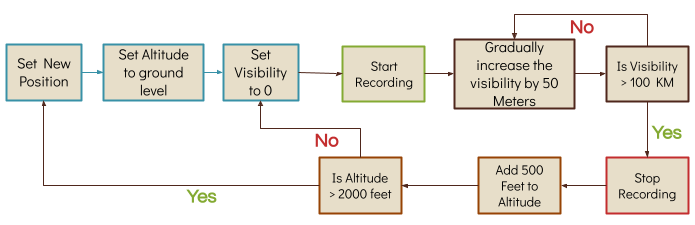
\includegraphics[width=250pt]{imgs/data_collection_pipeline.png}}
\caption{Automatic Dataset Collection Process using X-Plane 11}
\label{fig:data_collection_process}
\end{figure}
 

The collected images are automatically labeled into five discrete bins, each tailored to specific \href{https://www.faa.gov/air_traffic/publications/atpubs/aim_html/}{FAA requirements}. This categorization is based on visibility conditions and regulations relevant to both ground-based and aerial environments. The designated bins serve as the basis for the five labels utilized in training our DL models. 
We report the classes (bins) specifications and the corresponding counts in Table~\ref{tab:vis_img_count}.


\begin{figure}
  \centering
  \begin{subfigure}[b]{0.15\textwidth}
    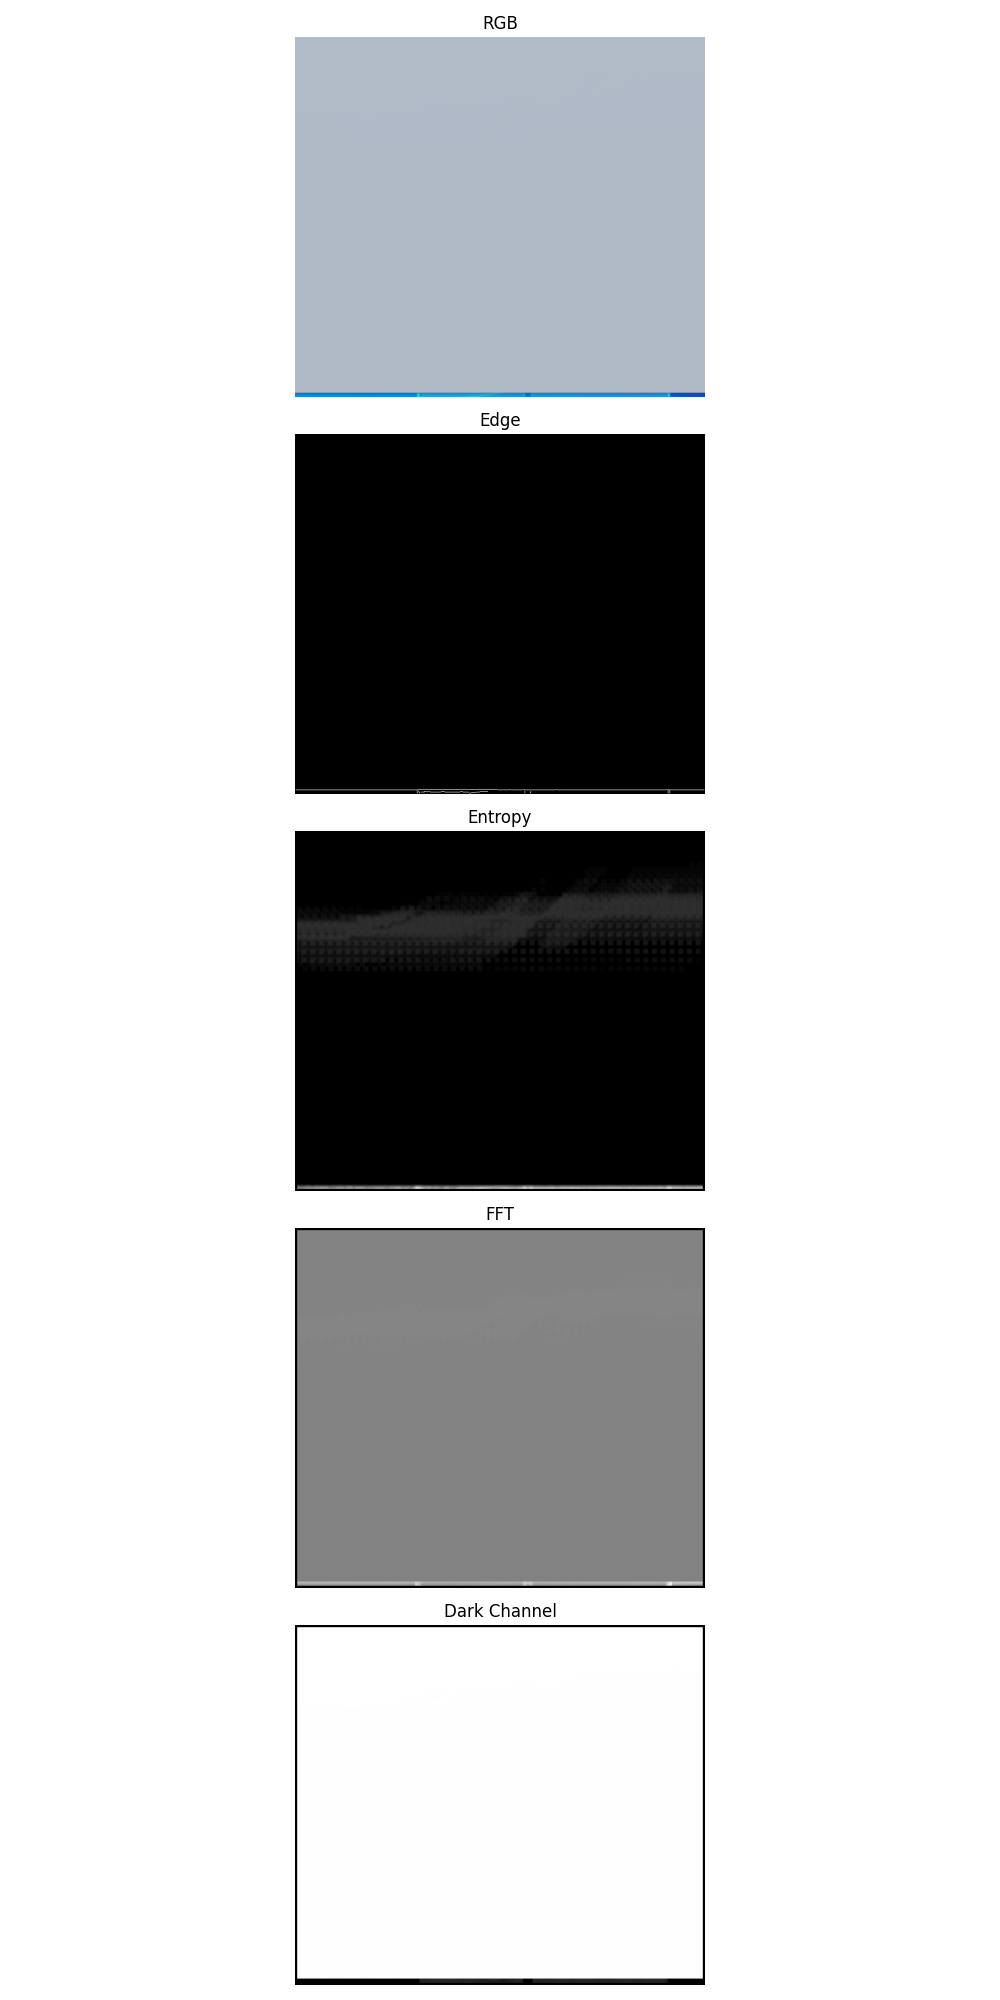
\includegraphics[width=\textwidth, trim={7.5cm 0cm 7.5cm 0cm},clip]{imgs/examples/exp_0_featuresMiles_0.12427454732996136_featuresM_200_features.png}
    \label{subfig:bin0}
        \caption{}
  \end{subfigure}
  \begin{subfigure}[b]{0.15\textwidth}
    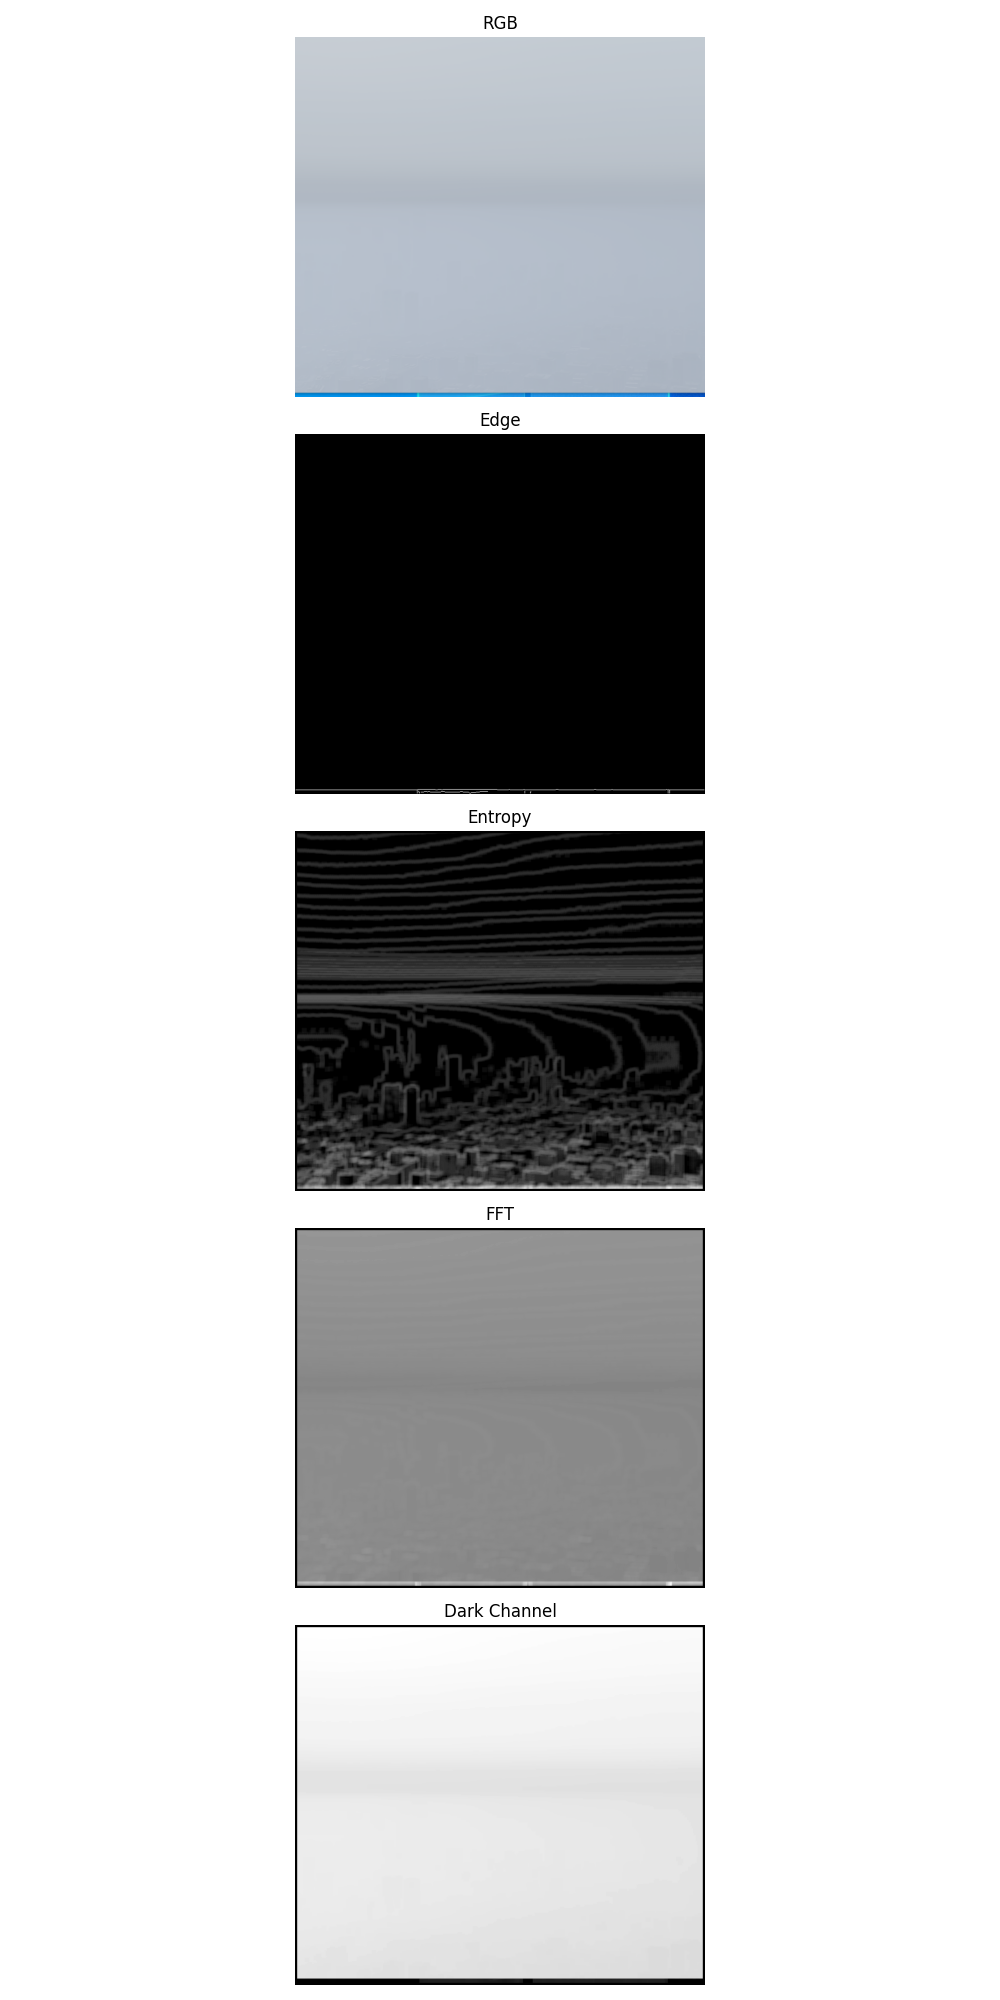
\includegraphics[width=\textwidth, trim={7.5cm 0 7.5cm 0},clip]{imgs/examples/exp_0_featuresMiles_0.9320591049747102_featuresM_1500_features.png}
    \label{subfig:bin1}
    \caption{}
  \end{subfigure}
  % Add the subfigrow environment here
    \begin{subfigure}[b]{0.15\textwidth}
      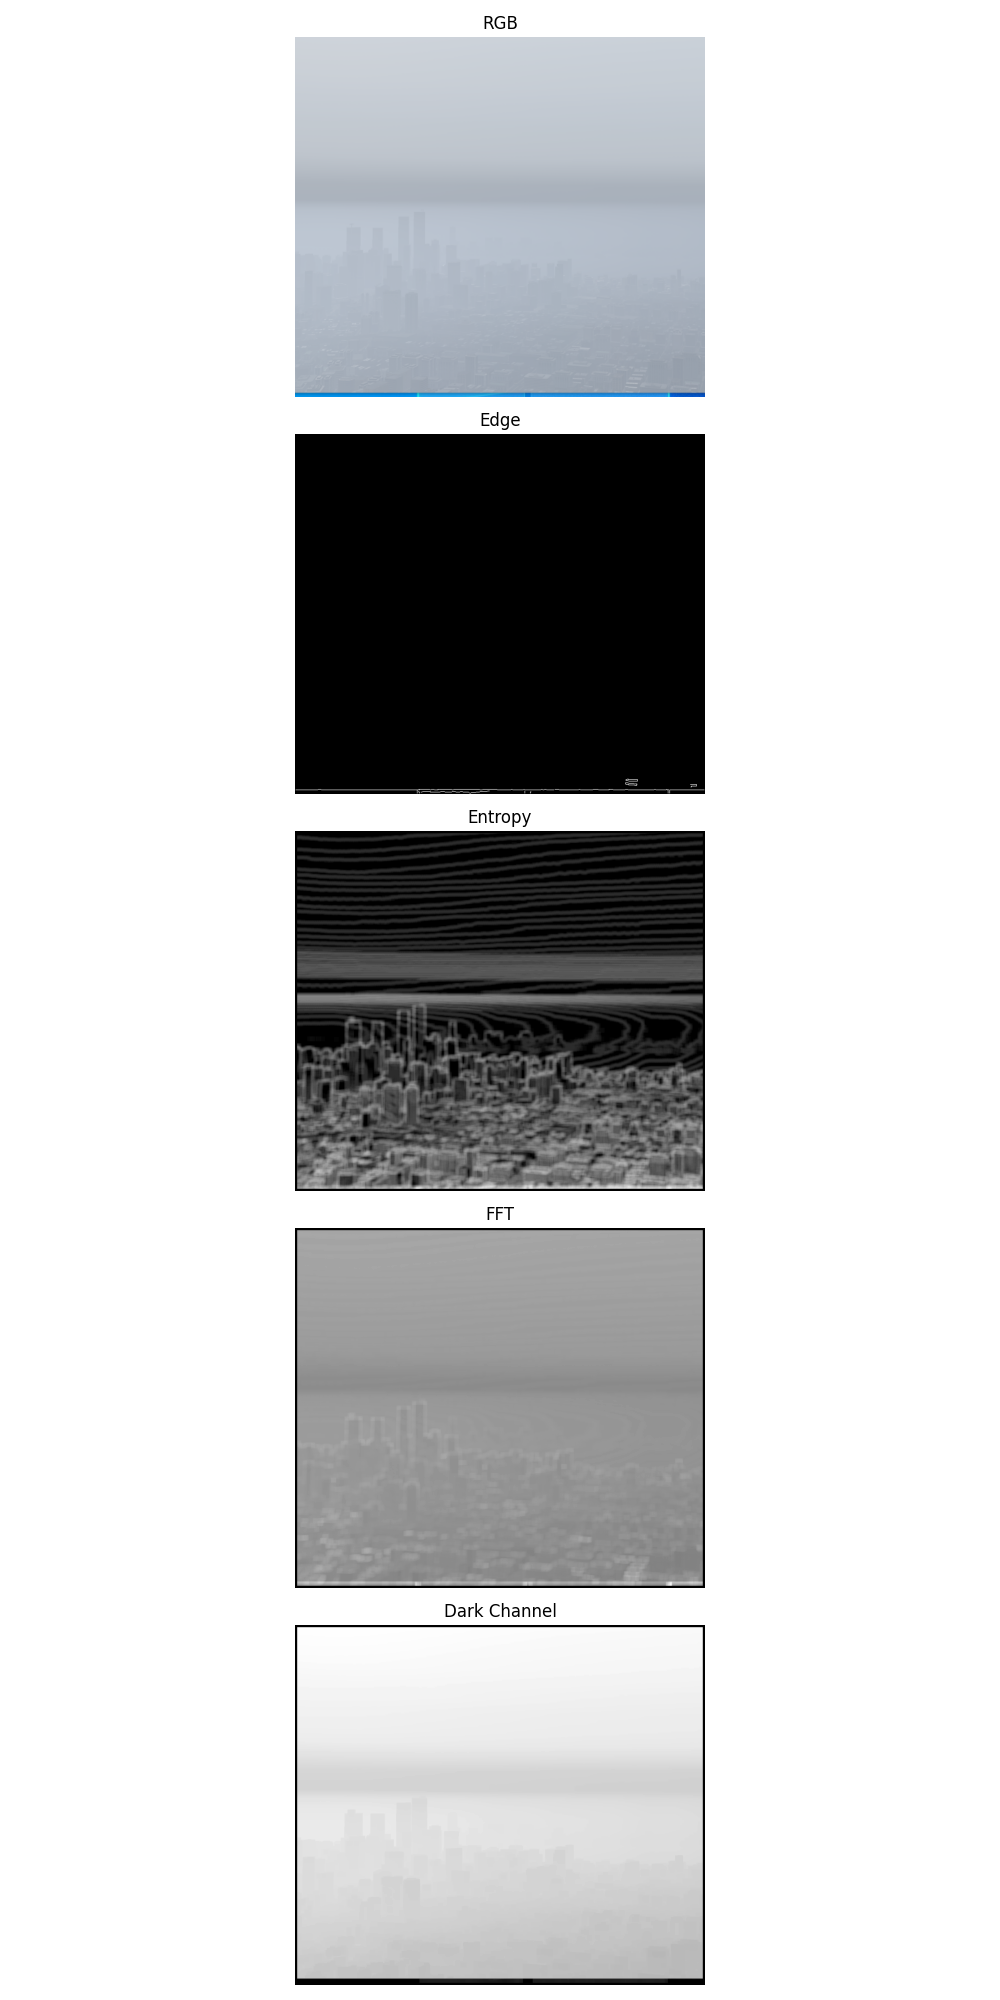
\includegraphics[width=\textwidth, trim={7.5cm 0 7.5cm 0},clip]{imgs/examples/exp_0_featuresMiles_1.8951868467819106_featuresM_3050_features.png}
      \label{subfig:bin2}
          \caption{}
    \end{subfigure}
    \begin{subfigure}[b]{0.15\textwidth}
      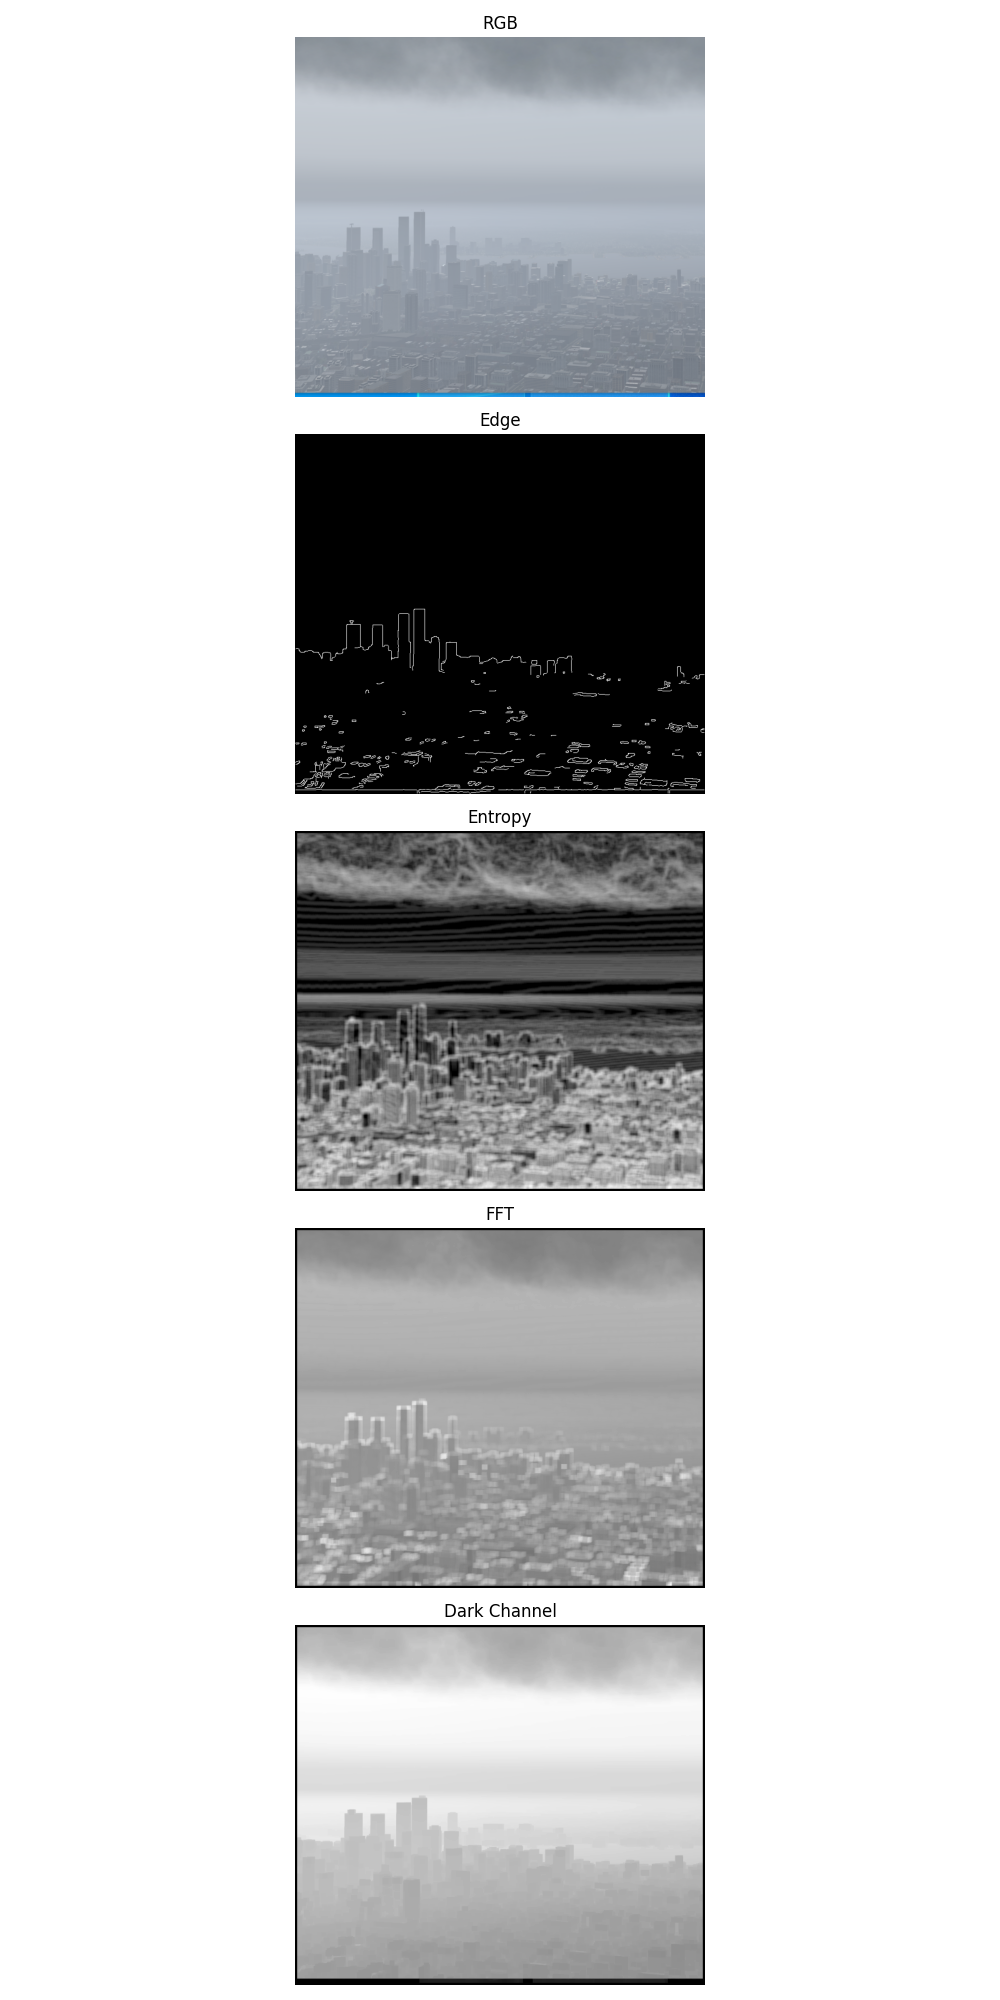
\includegraphics[width=\textwidth, trim={7.5cm 0 7.5cm 0},clip]{imgs/examples/exp_0_featuresMiles_4.038922788223744_featuresM_6500_features.png}
      \label{subfig:bin3}
          \caption{}
    \end{subfigure}
    \begin{subfigure}[b]{0.15\textwidth}
      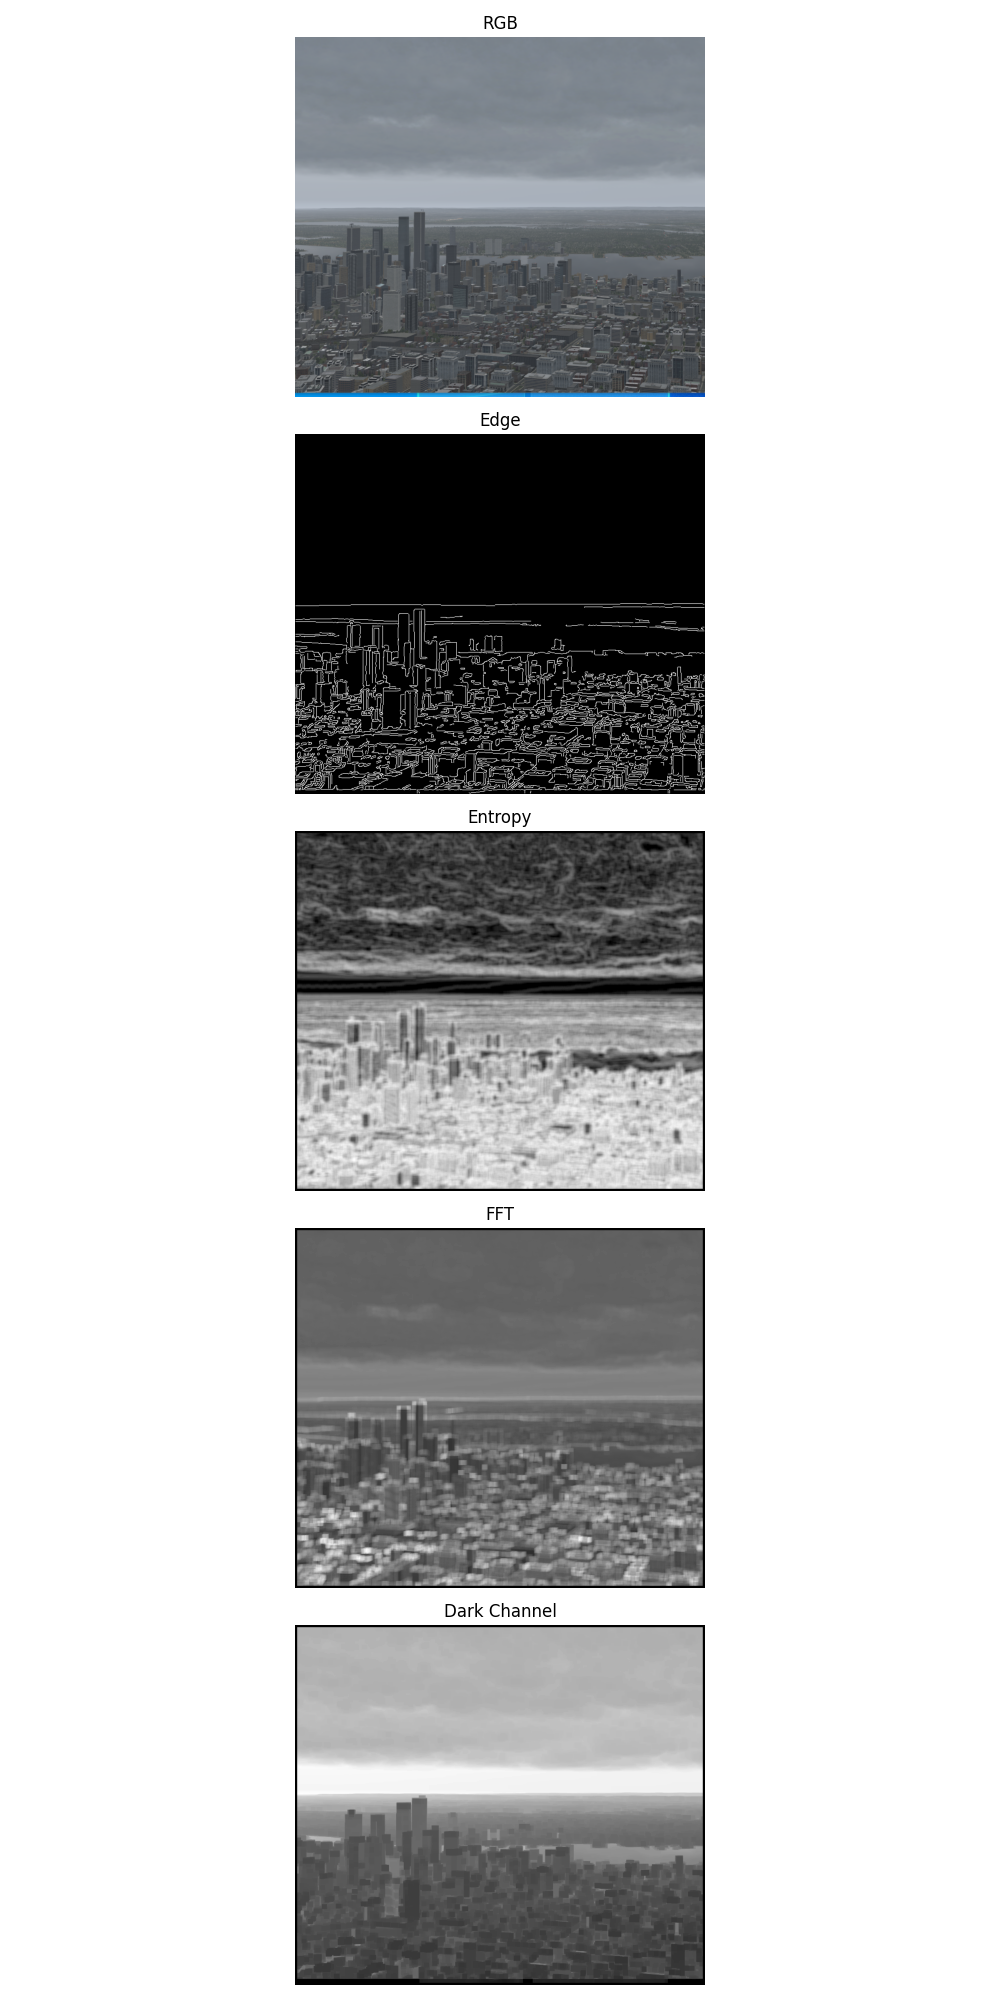
\includegraphics[width=\textwidth, trim={7.5cm 0 7.5cm 0},clip]{imgs/examples/exp_0_featuresMiles_46.1462462872979_featuresM_74265_features.png}
      \label{subfig:bin4}
          \caption{}
    \end{subfigure}
  
  \caption{We show the impact of visibility on the multiple modalities for the 6N7 Sealane 01 View. Each row shows one modality: RGB, edge map, entropy map, FFT magnitude, and dark channel prior. Each column refers to a visibility bin: (a) visibility of $< 0.5$ mile, (b) visibility range $(0.5, 1]$ miles, (c) visibility range $(1, 3]$ miles, (d) visibility range $(3, 5]$ miles, and (e) Visibility of $> 5$ miles. }
  \label{fig:impact_vis_deg_features}
\end{figure}


\begin{table}[htbp]
\centering
\caption{Visibility Categories and Images Count}
\label{tab:vis_img_count}
\begin{tabular}{|l|l|l|l|}
\hline
Category & Visibility in miles  & Visibility in meters & Count  \\ \hline
4        & $\geq$ 5 miles             &     $\geq$ 8046.72m                 & 67002  \\ \hline
3        & 3 to 5 miles         &      4828.03m to  8046.72m        & 19584  \\ \hline
2        & 1 to 3 miles         &            1609.34m to 4828.03m         & 19648  \\ \hline
1        & 0.5 miles to 1 mile  &               804.672m to 1609.34m      & 4928  \\ \hline
0        & $\leq$ 0.5 mile   &     $\leq$ 804.672m                 & 4938  \\ \hline
        &    &                      &  116100  \\ \hline
\end{tabular}
\end{table}


\subsubsection{Modalities}
\label{modalities}
\textbf{Monocular Depth Estimation:}

In our approach, we used the Omnidata toolkit to extract depth maps from monocular images \cite{eftekhar2021omnidata, ranftl2021vision}. This toolkit provides a comprehensive and scalable method for depth estimation, essential for understanding the spatial arrangement in a scene. The generated depth maps offer a pixel-wise measurement of distance from the viewpoint, aiding in the accurate representation of the three-dimensional structure of the scene. 

While depth maps offer valuable information, the models employed to generate them exhibit a notable limitation when applied to our data. The training methodology involves masking the sky and exclusively considering the ground before depth estimation. This approach may pose challenges with certain images in our dataset, as they are collected at varying altitudes.

\textbf{Normal Surface Estimation:}

Alongside depth maps, we also used the Omnidata toolkit for normal surface estimation \cite{eftekhar2021omnidata}. This modality provides information about the orientation of surfaces in the image, which is crucial for understanding the geometric properties of the scene. Unlike depth estimation, this modality estimator considers both sky and ground details.


\textbf{Entropy Map:}

We incorporate an image entropy map as a modality to enhance the model's sensitivity to changes in visibility, especially in low-visibility conditions. The entropy map quantifies the amount of information present in different regions of an image. 
% We report the procedure implemented to generate the Entropy Maps in Algorithm \ref{alg:entropy_map}.


% \begin{algorithm}[htbp]
% \caption{Calculate Entropy Map}\label{alg:entropy_map}
% \begin{algorithmic}[1]
% \Require An image $I$ represented as a 2D array, window size $w$
% \Ensure Entropy map $E$ of the same dimensions as $I$
% \State $E \gets \text{zeros\_like}(I)$ \Comment{Initialize entropy map $E$ with zeros}
% \State $rows, cols \gets$ dimensions of $I$ \Comment{Get the number of rows and columns of $I$}
% \For{$i \gets 0$ \textbf{to} $rows - w$} \Comment{Iterate over rows}
%     \For{$j \gets 0$ \textbf{to} $cols - w$} \Comment{Iterate over columns}
%         \State $window \gets I[i : i+w, j : j+w]$ \Comment{Extract $w \times w$ window from $I$}
%         \State $hist \gets \text{calculateHistogram}(window)$ \Comment{Calculate histogram of the window}
%         \State $hist \gets hist / \text{sum}(hist)$ \Comment{Normalize histogram}
%         \State $entropy \gets -\sum (hist \cdot \log_2(hist + \epsilon))$ \Comment{Compute entropy}
%         \State $E[i + \frac{w}{2}, j + \frac{w}{2}] \gets entropy$ \Comment{Assign entropy to center of window}
%     \EndFor
% \EndFor
% \State \Return $E$ \Comment{Return the computed entropy map}
% \end{algorithmic}
% \end{algorithm}


\textbf{Edge Detection:}

Edge detection is another key modality well-suited for scenarios involving long-range visibility where defining objects and scene boundaries is critical. By highlighting the contours and edges within the images, this modality aids in delineating shapes and structures, thus providing a clear distinction between different objects and features in the scene. 


\begin{figure}
    \centering
% Mean of Dark Channel Prior vs Visibility
    \begin{subfigure}[b]{0.4\textwidth}
        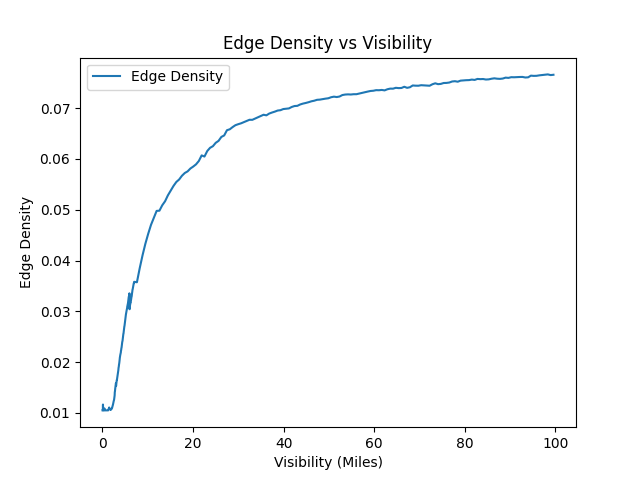
\includegraphics[width=\textwidth]{imgs/edge_density_vs_visibility.png}
    
    \end{subfigure}
    % Mean of Dark Channel Prior vs Visibility
    \begin{subfigure}[b]{0.4\textwidth}
        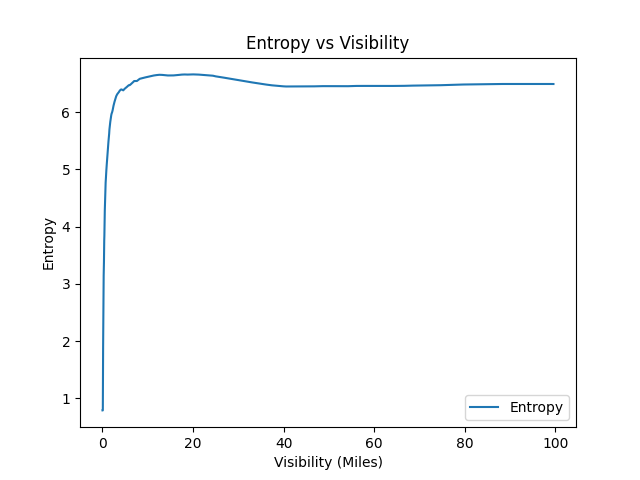
\includegraphics[width=\textwidth]{imgs/entropy_vs_visibility.png}
    \end{subfigure}
    % Mean of Edge Density vs Visibility
    \begin{subfigure}[b]{0.4\textwidth}
    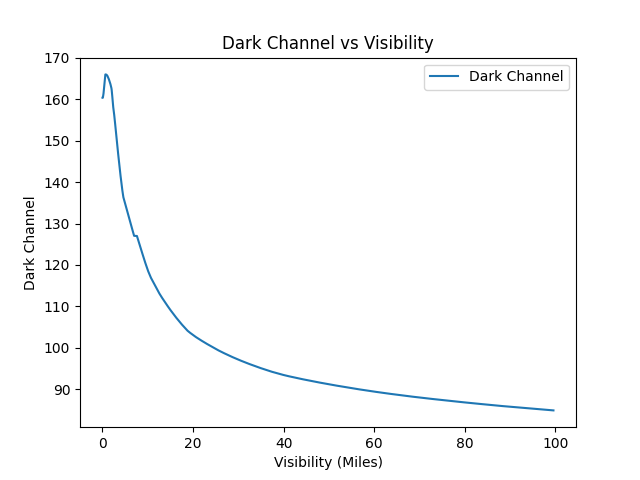
\includegraphics[width=\textwidth]{imgs/dark_channel_vs_visibility.png}
        
    \end{subfigure}
    % Mean of FFT Magnitude vs Visibility
    \begin{subfigure}[b]{0.4\textwidth}
        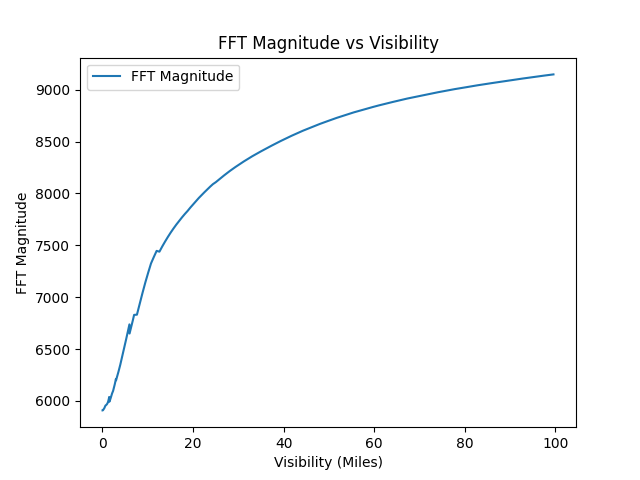
\includegraphics[width=\textwidth]{imgs/fft_magnitude_vs_visibility.png}
    \end{subfigure}
    \caption{Impact of Visibility Degradation on Edge Density (a), Entropy map (b), Dark Channel Prior (c), and FFT Magnitude (d) vs Visibility in Miles}
    \label{fig:mean_of_features}
\end{figure}

 In Figures~\ref{fig:impact_vis_deg_features}, \ref{fig:mean_of_features}, we show the impact of visibility degradation on various modalities of the same scenery. Each row shows one modality, while each column refers to a visibility bin.
\subsection{Fusing Modalities}
Numerous methods have been proposed in the literature for fusing different modalities and multiple stream networks \cite{akkus2023multimodal, radford2021learning, jia2021scaling}. These methods range from simple concatenation of different inputs from the input space to fusion at different levels of the model architecture. 

Early fusion \cite{huang_fusion_2020}, where we concatenate or preprocess all input streams in the input space, then feed it to a single feature extractor which extracts as much information as possible before feeding it to a decoder, classifier head, or projection head. While this method is the simplest method one can use to fuse different modalities, it has many limits where the feature-extracted model might learn to ignore most of the modalities from the early layers and be dominated by only one modality.

Another approach, widely used in the literature, involves feeding the different modalities into separate encoder layers before fusing all the extracted embeddings \cite{huang_fusion_2020}. In this approach, the model learns to extract useful features from each modality before they are fused, thus preventing one modality from dominating the feature space. But one of the biggest benefits of using this type of architecture is the ability to use recent advancements in representation learning, where each modality is processed through its own encoder, then using either contrastive learning to pre-train all the encoders to align together, or using the unsupervised representation learning where fusion happens in the between the encoder and decoder layer or right from the get-go.

Late fusion is another type of fusion \cite{huang_fusion_2020}, where each modality is passed through its own encoder, decoder, or any number of layers until the decision layer (e.g., binary classification). Fusion is then performed either by voting between different models or by taking the mean of the different decisions.

\subsubsection{Multimodal Fusion Methods}
In the literature, various techniques such as Tensor Fusion \cite{zadeh2017tensorfusionnetworkmultimodal}, Low-Rank Fusion \cite{liu2018efficientlowrankmultimodalfusion}, and attention \cite{NEURIPS2021_76ba9f56} have been proposed \. Although each method has its own advantages and disadvantages, self-attention has emerged as the cornerstone for many recent large-scale methods. While it requires more training data, its computation is significantly low compared to methods like tensor fusion.


\subsubsection{SeeNN Multimodal Fusion Framework}

\label{subsub:proposed}


\begin{figure}
    \centering
    \begin{subfigure}[b]{0.64\textwidth}
        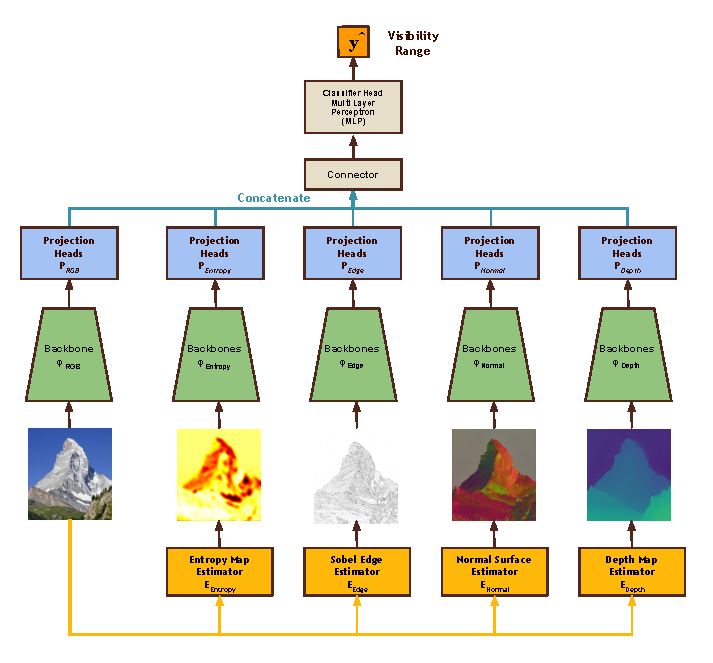
\includegraphics[width=\textwidth]{imgs/SeeNN_Expanded.pdf}
    \caption{}
    \end{subfigure}
    \begin{subfigure}[b]{0.2\textwidth}
        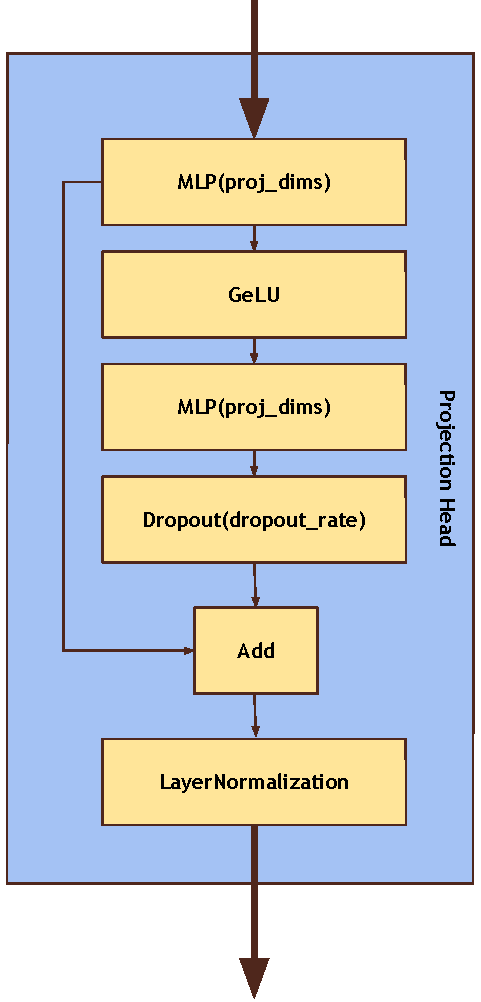
\includegraphics[width=\textwidth]{imgs/Projection Head.pdf}
    \label{fig:projection_head}
        \caption{}
    \end{subfigure}
\caption{
(a) SeeNN Framework: The framework first extracts features (entropy map, surface normals map, edge map, depth map) from the input image. Separate encoders $\phi_{m}(\cdot)$ ($\phi_{m}(\cdot)$ denotes modality encoders) process these features followed by a projection head (b), followed by fusion of these features through a Connector and prediction via a classifier $\mathbf{\hat{y}}$.
(b) Projection Head: The input vector is transformed by an MLP (Multi-Layer Perceptron) with a non-linear activation function (GeLU) and dropout for regularization.
}
\label{fig:seeeNN}
\end{figure}

The proposed SeeNN framework (Figure~\ref{fig:seeeNN}) integrates multimodal DL techniques to process the images alongside the multiple modalities. 
First, each input RGB image \( I \) undergoes a series of transformations through modality estimators to produce a depth map \( E_d(I) \), a normal surface map \( E_n(I) \), an edge detection map \( E_e(I) \), and an entropy map \( E_s(I) \). Each of these modalities captures distinct characteristics of the input, providing diverse perspectives on the image's content.

Let $m$ denote one of the modalities (generated depth map $depth$, normal surface $normal$, entropy map $entropy$, edge map $edge$, and RGB image $rgb$). We implement different backbone models $\Phi_{m}(\cdot)$ for each modality input $X_m$. 
We use DenseNet121 \cite{huang_densely_2018} as the architecture for all $\Phi_{m}$ and we feed the resulted embedding from each encoder to a projection head $P_m$ which consists of an MLP with a non-linear
activation function (GeLU) and dropout for regularization, followed by a layer normalization which is a crucial step to align the feature representations, mitigating the risk of dominance by any single modality due to varying magnitudes of feature values, then we obtain a feature vector \( F_m \).

We apply this process to RGB image $X_{rgb}$, depth \( X_{depth} \), normal surface  \( X_{normal} \), entropy  \( X_{entropy} \), and edge map \( X_{edge} \) to obtain $F_{rgb}$, $F_{depth}$, $F_{normal}$, $F_{entropy}$, $F_{edge}$, respectively. 

Following projection heads, the SeeNN framework concatenates these embeddings into a single, comprehensive feature vector \( F \). 
The concatenation is represented as \( F = [F_{rgb}, F_{depth}; F_{normal}; F_{entropy}; F_{edge}] \), which is then fed to the connector $C$ that is responsible for fusing these modalities.
We then apply an MLP classifier head to get the final prediction $\hat{y}$.  

When it comes to the connector, we primarily used two methods. The first method involves passing the flattened $F$ directly to the MLP, which involves a simple fusion of the different features. The second method utilizes an attention block to perform self-attention on $F$, followed by flattening the output and feeding it to the MLP head.


\subsubsection{Experimental Setup}
For our study, we use our collected dataset, SeeSet v1 \ref{sec:seeset}, made of 320 distinct views collected across 20 locations with different land covers, each with visibility ranging from 0 to 100 miles. We split the dataset into two subsets using the holdout approach, where we select all the views from specific locations, and hid them from the model during validation, to ensure that our model doesn't overfit the sceneries and vegetation and learn to estimate the visibility based on the degradation of the image \cite{Bouhsine2022}. This resulted in $100,350$ instances for training and $15,750$ for validation. Each image in the dataset is preprocessed to an input shape of $224 \times 224$ pixels.

We leverage the Omnidata models to preprocess RGB images and export the estimated Depth Map and the Normal Surface \cite{eftekhar2021omnidata}, which is based on the DPT-Hybrid architecture \cite{ranftl2021vision} and is similar to the approach taken in the literature to generate pseudo labels from RGB to pre-train multimodal models \cite{bachmann2022multimae, wang2024largescale}. 
For the other modalities, i.e., edge map and entropy map, the RGB images are initially processed through the hand-made estimators (Figure~\ref{fig:seeeNN}).

We train all models for 100 epochs and we use the Adam optimizer with a learning rate of $0.001$. For all models, we set the batch size to $32$.

\section{Results and Discussion}
\label{sec:results}

This section presents the experimental results of our study. We begin by describing the performance of a unimodal RGB-based model, followed by a detailed analysis of the multimodal SeeNN framework. The discussion encompasses a comparative analysis of different fusion strategies, an examination of model performance through confusion matrices, and a consideration of computational costs and dataset limitations.

\subsection{Unimodal Model Performance}

A baseline model was established using only the RGB modality. This unimodal model achieved an overall accuracy of 87.92\% on the validation set. This performance, while reasonable, highlights the inherent limitations of relying on a single data source, particularly when tested on previously unseen views. To ensure the robustness of our evaluation and prevent data leakage, we employed a strict holdout validation strategy, as described in the Experimental Setup, where entire geographical locations were withheld from the training set. This rigorous approach prevents the model from overfitting to specific sceneries and provides a more realistic assessment of its generalization capabilities.

\subsection{Multimodal Model Performance}

In contrast to the unimodal baseline, the multimodal models developed within the SeeNN framework demonstrated a significant improvement in performance. As shown in Table~\ref{tab:res_table} and Figure~\ref{fig:conf_mats}, the fusion of multiple modalities resulted in a substantial increase in prediction accuracy, with gains of up to 10 percentage points.

For instance, a model combining RGB and Depth modalities, using a simple concatenation connector, achieved an accuracy of 97.57\%. The highest performing model, which fused all five modalities (RGB, Entropy, Edge, Depth, and Normal Surface) using a self-attention connector, reached an impressive validation accuracy of 97.63\%. These results strongly support the hypothesis that integrating diverse data sources enables the model to form a more comprehensive and robust understanding of the atmospheric conditions, leading to more accurate visibility estimations.

\begin{table*}
\centering
\caption{Ablation study comparing the performance of different modality combinations and fusion connectors. The highest accuracy for each connector type is highlighted in bold.}
\label{tab:res_table}
\begin{tabular}{@{}lccccccr@{}}
\toprule
Connector & RGB & Entropy & Edge & Depth &  Normal Surface  & \# Trainable Params. & Val. Acc. (\%)  \\
\midrule
Unimodal & \checkmark &  &  &  &   & 7M &  87.92  \\
\midrule
\multirow{5}{*}{Concatenate}& \checkmark & \checkmark &  &  &   & 14M &  96.40  \\
& \checkmark &   & \checkmark &  &   & 14M & 96.53   \\
& \checkmark &  &  & \checkmark &   & 14M &   \textbf{97.57}  \\
& \checkmark &  &  & \checkmark & \checkmark  & 21M &   97.14  \\
& \checkmark & \checkmark & \checkmark  & \checkmark & \checkmark  & 38M & 96.30  \\
\midrule
\multirow{4}{*}{Self-Attention} & \checkmark &   & \checkmark &  &   & 14M & 96.86  \\
& \checkmark &  &  & \checkmark &   & 14M &   96.31  \\
& \checkmark &  &  & \checkmark & \checkmark  & 21M &   97.47  \\
& \checkmark & \checkmark & \checkmark  & \checkmark & \checkmark  & 38M & \textbf{97.63}  \\
\bottomrule
\end{tabular}
\end{table*}

\subsection{Analysis of Misclassifications}

The confusion matrices presented in Figure~\ref{fig:conf_mats} provide further insight into the performance of the top-performing multimodal models. While the overall accuracy is high, the models exhibit some difficulty in distinguishing between adjacent visibility categories. Specifically, there is a tendency to misclassify instances of "Class 3" (3 to 5 miles visibility) as "Class 4" (>= 5 miles visibility). This suggests that the visual cues differentiating these two classes are subtle and challenging for the models to discern.

Interestingly, the combination of RGB and Depth modalities yielded improved performance for this specific class, indicating that depth information is particularly valuable for resolving ambiguity in this visibility range. Future work could explore the integration of additional modalities or the development of more sophisticated fusion mechanisms to address this specific challenge.

\begin{figure}
    \centering
    \begin{subfigure}[b]{0.4\textwidth}
    %The matrix in numbers
%Horizontal target class
%Vertical output class
\def\myConfMat{{
{669,   3,   0,   0,    0},  %row 1
{  3,  657,  0,   0,    0},  %row 2
{   0,  12, 2638,  85,    33},  %row 3
{   0,   0,  50, 2368,   56},  %row 4
{   0,   0,   0,  132, 8941},  %row 5
}}

\def\classNames{{"$0$","$1$","$2$","$3$","$4$"}} %class names. Adapt at will

\def\numClasses{5} %number of classes. Could be automatic, but you can change it for tests.

\def\myScale{1.05} % 1.5 is a good scale. Values under 1 may need smaller fonts!
\begin{tikzpicture}[
    scale = \myScale,
    %font={\scriptsize}, %for smaller scales, even \tiny may be useful
    ]

\tikzset{vertical label/.style={rotate=90,anchor=east}}   % usable styles for below
\tikzset{diagonal label/.style={rotate=45,anchor=north east}}

\foreach \y in {1,...,\numClasses} %loop vertical starting on top
{
    % Add class name on the left
    \node [anchor=east] at (0.4,-\y) {\pgfmathparse{\classNames[\y-1]}\pgfmathresult}; 
    
    \foreach \x in {1,...,\numClasses}  %loop horizontal starting on left
    {
%---- Start of automatic calculation of totSamples for the column ------------   
    \def\totSamples{0}
    \foreach \ll in {1,...,\numClasses}
    {
        \pgfmathparse{\myConfMat[\ll-1][\x-1]}   %fetch next element
        \xdef\totSamples{\totSamples+\pgfmathresult} %accumulate it with previous sum
        %must use \xdef fro global effect otherwise lost in foreach loop!
    }
    \pgfmathparse{\totSamples} \xdef\totSamples{\pgfmathresult}  % put the final sum in variable
%---- End of automatic calculation of totSamples ----------------
    
    \begin{scope}[shift={(\x,-\y)}]
        \def\mVal{\myConfMat[\y-1][\x-1]} % The value at index y,x (-1 because of zero indexing)
        \pgfmathtruncatemacro{\r}{\mVal}   %
        \pgfmathtruncatemacro{\p}{round(\r/\totSamples*100)}
        \coordinate (C) at (0,0);
        \ifthenelse{\p<50}{\def\txtcol{black}}{\def\txtcol{white}} %decide text color for contrast
        \node[
            draw,                 %draw lines
            text=\txtcol,         %text color (automatic for better contrast)
            align=center,         %align text inside cells (also for wrapping)
            fill=black!\p,        %intensity of fill (can change base color)
            minimum size=\myScale*10mm,    %cell size to fit the scale and integer dimensions (in cm)
            inner sep=0,          %remove all inner gaps to save space in small scales
            ] (C) {\r\\\p\%};     %text to put in cell (adapt at will)
        %Now if last vertical class add its label at the bottom
        \ifthenelse{\y=\numClasses}{
        \node [] at ($(C)-(0,0.75)$) % can use vertical or diagonal label as option
        {\pgfmathparse{\classNames[\x-1]}\pgfmathresult};}{}
    \end{scope}
    }
}
%Now add x and y labels on suitable coordinates
\coordinate (yaxis) at (-0.2,0.3-\numClasses/2);  %must adapt if class labels are wider!
\coordinate (xaxis) at (0.5+\numClasses/2, -\numClasses-1.2); %id. for non horizontal labels!
\node [vertical label] at (yaxis) {Predicted Label};
\node []               at (xaxis) {True Label};
\end{tikzpicture}

\caption{All modalities with the Self-Attention Block}

    \caption{All Modalities (Self-Attention)}
    \end{subfigure}
    \begin{subfigure}[b]{0.4\textwidth}
        %The matrix in numbers
%Horizontal target class
%Vertical output class
\def\myConfMat{{
{664,   0,   0,   0,    0},  %row 1
{  8,  663,  0,   0,    0},  %row 2
{   0,  9, 2618,  143,    114},  %row 3
{   0,   0,  70, 2368,   61},  %row 4
{   0,   0,   0,  177, 8855},  %row 5
}}

\def\classNames{{"$0$","$1$","$2$","$3$","$4$"}} %class names. Adapt at will

\def\numClasses{5} %number of classes. Could be automatic, but you can change it for tests.

\def\myScale{1.05} % 1.5 is a good scale. Values under 1 may need smaller fonts!
\begin{tikzpicture}[
    scale = \myScale,
    %font={\scriptsize}, %for smaller scales, even \tiny may be useful
    ]

\tikzset{vertical label/.style={rotate=90,anchor=east}}   % usable styles for below
\tikzset{diagonal label/.style={rotate=45,anchor=north east}}

\foreach \y in {1,...,\numClasses} %loop vertical starting on top
{
    % Add class name on the left
    \node [anchor=east] at (0.4,-\y) {\pgfmathparse{\classNames[\y-1]}\pgfmathresult}; 
    
    \foreach \x in {1,...,\numClasses}  %loop horizontal starting on left
    {
%---- Start of automatic calculation of totSamples for the column ------------   
    \def\totSamples{0}
    \foreach \ll in {1,...,\numClasses}
    {
        \pgfmathparse{\myConfMat[\ll-1][\x-1]}   %fetch next element
        \xdef\totSamples{\totSamples+\pgfmathresult} %accumulate it with previous sum
        %must use \xdef fro global effect otherwise lost in foreach loop!
    }
    \pgfmathparse{\totSamples} \xdef\totSamples{\pgfmathresult}  % put the final sum in variable
%---- End of automatic calculation of totSamples ----------------
    
    \begin{scope}[shift={(\x,-\y)}]
        \def\mVal{\myConfMat[\y-1][\x-1]} % The value at index y,x (-1 because of zero indexing)
        \pgfmathtruncatemacro{\r}{\mVal}   %
        \pgfmathtruncatemacro{\p}{round(\r/\totSamples*100)}
        \coordinate (C) at (0,0);
        \ifthenelse{\p<50}{\def\txtcol{black}}{\def\txtcol{white}} %decide text color for contrast
        \node[
            draw,                 %draw lines
            text=\txtcol,         %text color (automatic for better contrast)
            align=center,         %align text inside cells (also for wrapping)
            fill=black!\p,        %intensity of fill (can change base color)
            minimum size=\myScale*10mm,    %cell size to fit the scale and integer dimensions (in cm)
            inner sep=0,          %remove all inner gaps to save space in small scales
            ] (C) {\r\\\p\%};     %text to put in cell (adapt at will)
        %Now if last vertical class add its label at the bottom
        \ifthenelse{\y=\numClasses}{
        \node [] at ($(C)-(0,0.75)$) % can use vertical or diagonal label as option
        {\pgfmathparse{\classNames[\x-1]}\pgfmathresult};}{}
    \end{scope}
    }
}
%Now add x and y labels on suitable coordinates
\coordinate (yaxis) at (-0.2,0.3-\numClasses/2);  %must adapt if class labels are wider!
\coordinate (xaxis) at (0.5+\numClasses/2, -\numClasses-1.2); %id. for non horizontal labels!
\node [vertical label] at (yaxis) {Predicted Label};
\node []               at (xaxis) {True Label};
\end{tikzpicture}

\caption{All modalities with the concatenate connector}

        \caption{All Modalities (Concatenate)}
    \end{subfigure}
    \\
    \begin{subfigure}[b]{0.4\textwidth}
        %The matrix in numbers
%Horizontal target class
%Vertical output class
\def\myConfMat{{
{660,   0,   0,   0,    0},  %row 1
{  12,  671,  41,   0,    0},  %row 2
{   0,  1, 2540,  23,    0},  %row 3
{   0,   0,  107, 2524,   57},  %row 4
{   0,   0,   0,  141, 8973},  %row 5
}}

\def\classNames{{"$0$","$1$","$2$","$3$","$4$"}} %class names. Adapt at will

\def\numClasses{5} %number of classes. Could be automatic, but you can change it for tests.

\def\myScale{1.05} % 1.5 is a good scale. Values under 1 may need smaller fonts!
\begin{tikzpicture}[
    scale = \myScale,
    %font={\scriptsize}, %for smaller scales, even \tiny may be useful
    ]

\tikzset{vertical label/.style={rotate=90,anchor=east}}   % usable styles for below
\tikzset{diagonal label/.style={rotate=45,anchor=north east}}

\foreach \y in {1,...,\numClasses} %loop vertical starting on top
{
    % Add class name on the left
    \node [anchor=east] at (0.4,-\y) {\pgfmathparse{\classNames[\y-1]}\pgfmathresult}; 
    
    \foreach \x in {1,...,\numClasses}  %loop horizontal starting on left
    {
%---- Start of automatic calculation of totSamples for the column ------------   
    \def\totSamples{0}
    \foreach \ll in {1,...,\numClasses}
    {
        \pgfmathparse{\myConfMat[\ll-1][\x-1]}   %fetch next element
        \xdef\totSamples{\totSamples+\pgfmathresult} %accumulate it with previous sum
        %must use \xdef fro global effect otherwise lost in foreach loop!
    }
    \pgfmathparse{\totSamples} \xdef\totSamples{\pgfmathresult}  % put the final sum in variable
%---- End of automatic calculation of totSamples ----------------
    
    \begin{scope}[shift={(\x,-\y)}]
        \def\mVal{\myConfMat[\y-1][\x-1]} % The value at index y,x (-1 because of zero indexing)
        \pgfmathtruncatemacro{\r}{\mVal}   %
        \pgfmathtruncatemacro{\p}{round(\r/\totSamples*100)}
        \coordinate (C) at (0,0);
        \ifthenelse{\p<50}{\def\txtcol{black}}{\def\txtcol{white}} %decide text color for contrast
        \node[
            draw,                 %draw lines
            text=\txtcol,         %text color (automatic for better contrast)
            align=center,         %align text inside cells (also for wrapping)
            fill=black!\p,        %intensity of fill (can change base color)
            minimum size=\myScale*10mm,    %cell size to fit the scale and integer dimensions (in cm)
            inner sep=0,          %remove all inner gaps to save space in small scales
            ] (C) {\r\\\p\%};     %text to put in cell (adapt at will)
        %Now if last vertical class add its label at the bottom
        \ifthenelse{\y=\numClasses}{
        \node [] at ($(C)-(0,0.75)$) % can use vertical or diagonal label as option
        {\pgfmathparse{\classNames[\x-1]}\pgfmathresult};}{}
    \end{scope}
    }
}
%Now add x and y labels on suitable coordinates
\coordinate (yaxis) at (-0.2,0.3-\numClasses/2);  %must adapt if class labels are wider!
\coordinate (xaxis) at (0.5+\numClasses/2, -\numClasses-1.2); %id. for non horizontal labels!
\node [vertical label] at (yaxis) {Predicted Label};
\node []               at (xaxis) {True Label};
\end{tikzpicture}

\caption{RGB and Depth Map Model with the Concatenate Connector}

        \caption{RGB + Depth (Concatenate)}
    \end{subfigure}
    \begin{subfigure}[b]{0.4\textwidth}
        %The matrix in numbers
%Horizontal target class
%Vertical output class
\def\myConfMat{{
{635,   0,   0,   0,    0},  %row 1
{  37,  661,  0,   0,    0},  %row 2
{   0,  11, 2636,  52,    0},  %row 3
{   0,   0,  52, 2301,   307},  %row 4
{   0,   0,   0,  94, 8936},  %row 5
}}

\def\classNames{{"$0$","$1$","$2$","$3$","$4$"}} %class names. Adapt at will

\def\numClasses{5} %number of classes. Could be automatic, but you can change it for tests.

\def\myScale{1.05} % 1.5 is a good scale. Values under 1 may need smaller fonts!
\begin{tikzpicture}[
    scale = \myScale,
    %font={\scriptsize}, %for smaller scales, even \tiny may be useful
    ]

\tikzset{vertical label/.style={rotate=90,anchor=east}}   % usable styles for below
\tikzset{diagonal label/.style={rotate=45,anchor=north east}}

\foreach \y in {1,...,\numClasses} %loop vertical starting on top
{
    % Add class name on the left
    \node [anchor=east] at (0.4,-\y) {\pgfmathparse{\classNames[\y-1]}\pgfmathresult}; 
    
    \foreach \x in {1,...,\numClasses}  %loop horizontal starting on left
    {
%---- Start of automatic calculation of totSamples for the column ------------   
    \def\totSamples{0}
    \foreach \ll in {1,...,\numClasses}
    {
        \pgfmathparse{\myConfMat[\ll-1][\x-1]}   %fetch next element
        \xdef\totSamples{\totSamples+\pgfmathresult} %accumulate it with previous sum
        %must use \xdef fro global effect otherwise lost in foreach loop!
    }
    \pgfmathparse{\totSamples} \xdef\totSamples{\pgfmathresult}  % put the final sum in variable
%---- End of automatic calculation of totSamples ----------------
    
    \begin{scope}[shift={(\x,-\y)}]
        \def\mVal{\myConfMat[\y-1][\x-1]} % The value at index y,x (-1 because of zero indexing)
        \pgfmathtruncatemacro{\r}{\mVal}   %
        \pgfmathtruncatemacro{\p}{round(\r/\totSamples*100)}
        \coordinate (C) at (0,0);
        \ifthenelse{\p<50}{\def\txtcol{black}}{\def\txtcol{white}} %decide text color for contrast
        \node[
            draw,                 %draw lines
            text=\txtcol,         %text color (automatic for better contrast)
            align=center,         %align text inside cells (also for wrapping)
            fill=black!\p,        %intensity of fill (can change base color)
            minimum size=\myScale*10mm,    %cell size to fit the scale and integer dimensions (in cm)
            inner sep=0,          %remove all inner gaps to save space in small scales
            ] (C) {\r\\\p\%};     %text to put in cell (adapt at will)
        %Now if last vertical class add its label at the bottom
        \ifthenelse{\y=\numClasses}{
        \node [] at ($(C)-(0,0.75)$) % can use vertical or diagonal label as option
        {\pgfmathparse{\classNames[\x-1]}\pgfmathresult};}{}
    \end{scope}
    }
}
%Now add x and y labels on suitable coordinates
\coordinate (yaxis) at (-0.2,0.3-\numClasses/2);  %must adapt if class labels are wider!
\coordinate (xaxis) at (0.5+\numClasses/2, -\numClasses-1.2); %id. for non horizontal labels!
\node [vertical label] at (yaxis) {Predicted Label};
\node []               at (xaxis) {True Label};
\end{tikzpicture}

\caption{RGB and Depth Map Model with the Self-Attention Block}

        \caption{RGB + Depth (Self-Attention)}
    \end{subfigure}
    \caption{Confusion matrices for the top-performing multimodal models. The models show high accuracy but struggle with adjacent classes, particularly misclassifying Class 3 as Class 4.}
    \label{fig:conf_mats}
\end{figure}

\subsection{Discussion}

\subsubsection{Computational Cost and Deployment Considerations}

A critical consideration in the practical application of these models is the trade-off between performance and computational cost. While the model that fused all available modalities achieved the highest accuracy, it also has the highest computational overhead, requiring the execution of multiple modality estimators and backbone networks. When deploying such models, particularly on resource-constrained hardware such as embedded devices, it is essential to consider these limitations. The results suggest that a carefully selected subset of modalities (e.g., RGB and Depth) can provide a favorable balance between accuracy and efficiency.

\subsubsection{Dataset Limitations and Future Directions}

While the SeeSet V1 dataset addresses a significant gap in the availability of public, multi-view datasets for atmospheric visibility research, it has certain limitations. The diversity of landscapes and land covers could be expanded to enhance the model's generalizability. Future work should focus on enriching the dataset using the latest generation of flight simulators (e.g., Microsoft Flight Simulator, X-Plane 12), which offer near-photorealistic rendering and more sophisticated atmospheric models.

Further research should also explore advanced pre-training techniques to improve the quality of the learned feature representations. Many state-of-the-art multimodal systems leverage self-supervised or unsupervised pre-training on large-scale datasets, which has been shown to improve downstream task performance.

Finally, a deeper investigation into the impact of visibility degradation on the feature representations extracted by different network architectures is warranted. A thorough understanding of this relationship is crucial for improving the trustworthiness and reliability of these models in safety-critical, real-world applications.




\section{Conclusion}
\label{sec:conclusion}

In this paper, we have presented a novel multimodal deep learning framework, SeeNN, for the estimation of atmospheric visibility in challenging in-flight scenarios. Our work makes two primary contributions to the field.

First, we introduced the SeeNN framework, which effectively fuses information from RGB imagery, entropy maps, edge maps, depth maps, and normal surface maps. Our extensive experimental results demonstrate that this multimodal approach significantly outperforms traditional unimodal models that rely solely on RGB data. The superior performance of SeeNN underscores the value of integrating diverse data modalities to overcome the inherent ambiguities and limitations of single-source systems, thereby achieving more accurate and reliable visibility estimation.

Second, we have developed and released a comprehensive, open-source benchmark dataset for atmospheric visibility estimation. This dataset, a key contribution of our work, is distinguished by its diversity, encompassing a wide range of altitudes, land cover types, and visibility conditions. It provides a much-needed resource for the research community, enabling the robust training, validation, and comparative evaluation of visibility estimation algorithms.

Our empirical results show that the proposed multimodal framework offers substantial improvements in estimation accuracy over unimodal RGB methods. The release of our benchmark dataset addresses a critical gap in the field, providing a standardized platform for future research and development. We anticipate that this resource will catalyze further innovation in the domain, spurring the development of increasingly sophisticated multimodal deep learning techniques for atmospheric visibility estimation.

Future research could explore several promising avenues, including the integration of additional sensor modalities, the investigation of more advanced fusion architectures, and the application of our framework to related problems in atmospheric science. Furthermore, the potential for leveraging transfer learning and domain adaptation techniques in this context remains a compelling area for future investigation.

In conclusion, this work contributes to the growing body of research at the intersection of deep learning and atmospheric science, offering both methodological advancements and a valuable resource to the research community. As the field continues to evolve, we believe that multimodal approaches, such as the one presented in this paper, will play an increasingly pivotal role in addressing complex environmental perception tasks, with far-reaching implications for aviation safety and other domains.


\section*{Acknowledgments}

This research was supported by the Federal Aviation Administration (FAA). The authors wish to express their gratitude to the William J. Hughes Technical Center for providing the resources and support necessary for this work. The views, opinions, and/or findings contained in this paper are those of the authors and should not be construed as an official position, policy, or decision of the FAA, unless so designated by other documentation.
\bibliography{sample}




\end{document}
